\documentclass{article}

\usepackage[preprint]{nips_2018}
% to avoid loading the natbib package, add option nonatbib:
% \usepackage[nonatbib]{nips_2018}

\usepackage[utf8]{inputenc} % allow utf-8 input
% \usepackage[T1]{fontenc}    % use 8-bit T1 fonts
\usepackage{hyperref}       % hyperlinks
\usepackage{url}            % simple URL typesetting
\usepackage{booktabs}       % professional-quality tables
\usepackage{amsfonts}       % blackboard math symbols
\usepackage{nicefrac}       % compact symbols for 1/2, etc.
\usepackage{microtype}      % microtypography
\usepackage{amsmath}
\usepackage{float}
\usepackage{graphicx}
\usepackage{algorithm}
\usepackage{algpseudocode}
\usepackage{cleveref}       % this package must be loaded at the last
%\usepackage{subcaption}
\usepackage{subfigure}

\title{Lab1 Report}

\author{
  Chun Hung Lin \\
  \texttt{chlin3@kth.se}
  \And
  Yini Yang \\
  \texttt{yiniy@kth.se} \\
  \texttt{199504244188}
}

\begin{document}
\maketitle

% Quesiton 1
\section{Problem 1: The Maze and the Random Minotaur}
\subsection{Formulate the problem as an MDP}
This problem can be formulated as an MDP with finite horizon.
\newline

\textbf{State space:} \\
Here we use a pair of positions in the maze as a state. The state space $S$ can be described as follows:
$$S=\{S_i=(x_p,y_p,x_m,y_m)|i=0,\cdots,3135\}, \quad x_p,x_m\in [0,6],\  y_p,y_m\in [0,7]$$
where $(x_p,y_p)$ refers to the position of the person, while $(x_m,y_m)$ is the position of the Minotaur.
Here we can divide this state space into four part:
$$S=S_{unavailable}\cup S_{available}\cup S_{dead}\cup S_{escape}$$
where $S_{unavailable}=\{(x_p,y_p)\in wall\}$ refers to the states where the person is in the wall. 
$S_{dead}=\{S_i|x_p=x_m,y_p=y_m\}$ corresponds to the states where the person and minotaur are in the same position. 
$S_{escape}=\{S_i|(x_p,y_p)=exit,(y_p,y_m)\neq exit\}$ includes the states at which the person succeeds escaping.
And both $S_{dead}, S_{escape}$ are absorbing states.
\newline

\textbf{Action space:} \\
In this problem, the minotaur follows a random walk. The action space for the person is as below:
$$A=\{\textup{Up},\textup{Down},\textup{Left},\textup{Right},\textup{StandStill}\}$$
\newline

\textbf{Reward:} \\
The reward can be formulated as a function of $r: S\times A\rightarrow \mathbb{R}$.
$$r(s,:)=\left\{\begin{aligned}
 10 \quad &s\in S_{escape} \\
 -1 \quad &s\in S_{dead} \\
 0 \quad &\textup{otherwise}
\end{aligned}\right.$$
When the state is in $S_{escape}$, no matter what actions the person take, the reward will always be 10. 
While the state is in $S_{dead}$, the punishment will be $-1$ for whatever actions. 
For other available movement, there will be no reward or punishment.
\newline

\textbf{Transition probability:} \\
For the person, the policy is deterministic. In other words, given the current position and the action, the next position of the person is deterministic.
So for the state transition, the uncertainty comes from the minotaur. Thus the transition probability can be formulated as follows:
$$P_t(s_j|s_i,a)=\left\{\begin{aligned}
  &\frac{1}{|\textup{Aja}(s_{i_M})|} \quad &s_{j_M}\in \textup{Aja}(s_{i_M}) \\
  &1 \quad &S_i\in S_{dead}\cup S_{escape} \\
  &0 \quad &\textup{otherwise}
\end{aligned}\right.$$
where $s_{i_M}=(x_{i_m},y_{i_m})$ means the minotaur's position at state $i$, and $\textup{Aja}(s_{i_M})$ is the set of adjacent positions to $s_{i_M}$.
And when the environment has reached the absorbing state, it will always stay in this state.
\newline

\textbf{Objective funcion:} \\
This MDP is under a finite time horizon $T$. Thus the objective function can be formulated as the total rewards obtained in $T$ steps:
$$G_T=\mathbb{E}\left\{\sum_{t=1}^T r_t(s_t,a_t)\right\}$$

\subsection{Solve the problem for T=20}
One generated solution has been shown in Figure \ref{solution}.
The red arrows correspond to the person's route, while the blue ones refer to the minotaur's route.
In this solution, the person succeeds escaping when $t=17$.
\begin{figure}[h]
  \centering
  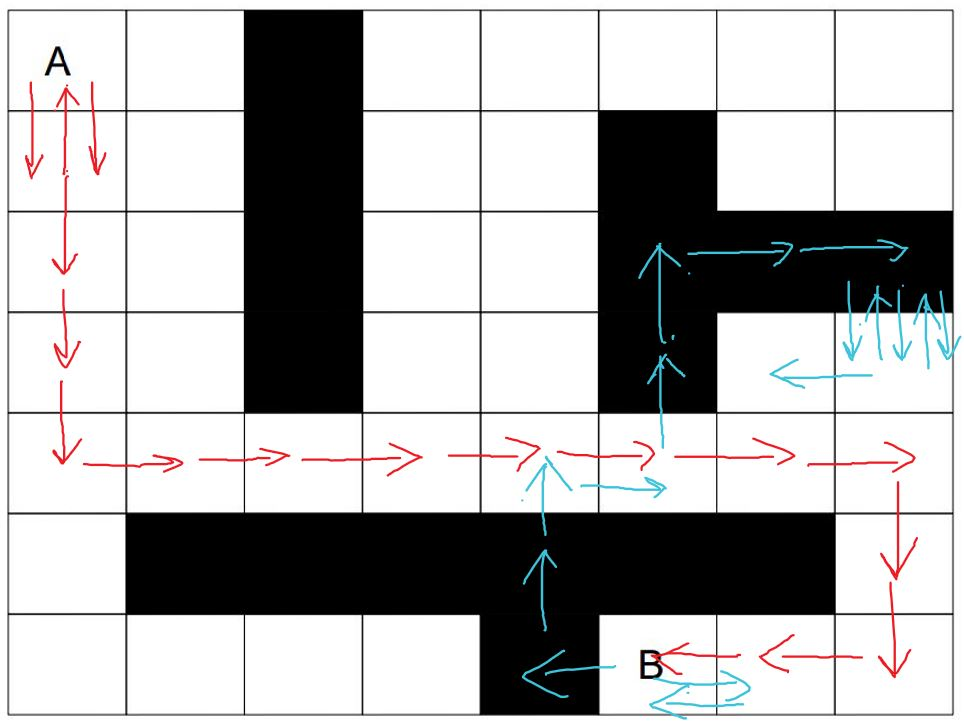
\includegraphics[scale=0.4]{solution.jpg}
  \caption{A generated solution for T=20. (Red trajectory: person, blue trajectory: minotaur.)}
  \label{solution}
\end{figure}

The maximal probability of exiting the maze has been estimated as a function of T. Here we consider both cases of whether the minotaur is allowed to stand still or not. 
The results for $T\in [1,30]$ are shown in Figure \ref{probability}.
\begin{figure}[H]
  \subfigure[Minotaur can not stand still.]{
    \begin{minipage}[t]{0.5\linewidth}
      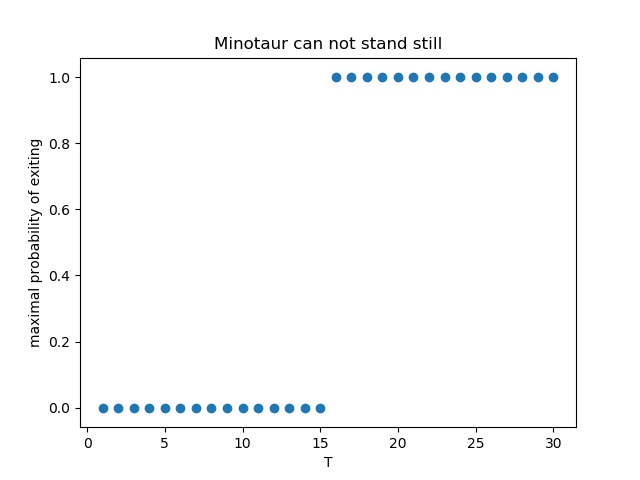
\includegraphics[scale=0.45]{no stand still.png}
      \centering
    \end{minipage}
  }
  \subfigure[Minotaur can stand still.]{
    \begin{minipage}[t]{0.5\linewidth}
      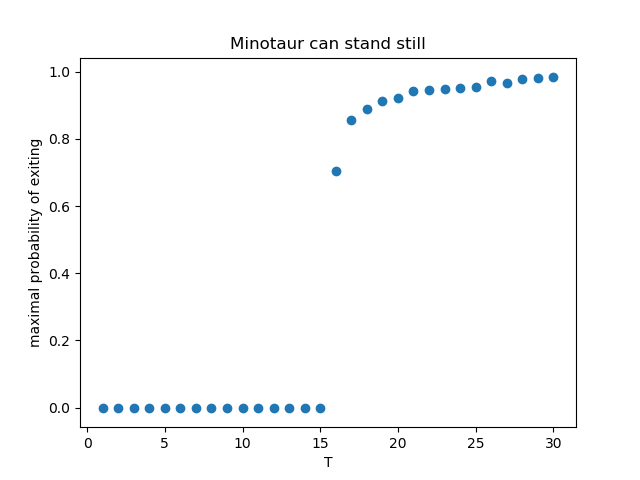
\includegraphics[scale=0.45]{stand still.png}
      \centering
    \end{minipage}
  }
  \caption{The probability of exiting the maze related to T.}
  \label{probability}
\end{figure}

For both cases, the exit probability for $T\leq 15$ is $0$. As the person need at least $15$ steps to arrive at exit even when there is not a minotaur.
When the minotaur is not allowed to stand still, the maximal probability for $T\geq 15$ is $1$. While in the other case, the maximal probability will gradually reach to 1 as $T$ increases.
When the minotaur stays in a position, the person will also keep still or move in an opposite direction to be as far as possible to the minotaur. 
Thus, under this condition, the person tends to use more time to exit. 
In other words, the maximal exiting probability with a standing still action will be a little bit less than that of the other case. 

\subsection{Modify MDP with infinite time horizon}
Under this condition, the time horizon is no longer finite. Instead, $T$ is infinite and follows the following geometric distribution:
$$P(T=t)=(1-p)^tp, \quad t=0,1,\cdots$$
where $p=\frac{1}{30}$. Therefore, when $t$ is increasing, the probability is decreasing. 
Thus, we can re-formulate this problem as a MDP with infinite time horizon and discounted rewards. The objective function is changed into:
$$G_{T\sim Geo(p)}=\mathbb{E}_{T\sim Geo(p)}\left\{\sum_{t=1}^{\infty}(1-p)^t r_t(s_t,a_t)\right\}$$
where $1-p=0.97$.
Other settings for this MDP are the same as before. And now we can use the value iteration(VI) algorithm to obtain the optimal policy.
After simulating 10000 games with the optimal policy obtained from VI, the estimated probability of exiting is $97.83\%$.
% Quesiton 2

% Quesiton 3
\section{Quesiton 3}

% Quesiton 4
\section{Quesiton 4}
\end{document}
